% AUTHOR: Diego Sarceno
% Last Update: 11.07.2020

\documentclass[11pt, spanish, letterpaper]{article} %tipo de documento

\usepackage[letterpaper]{geometry} %margenes
\geometry{verbose,tmargin=2.5cm,bmargin=2.5cm,lmargin=2cm,rmargin=2cm}
\usepackage{amsmath,amsthm,amssymb} %modos matemáticos y  simbolos
\usepackage{latexsym,amsfonts} %simbolos matematicos
\usepackage{cancel} %hacer la linea que cancela las ecuaciones
\usepackage[spanish, es-noshorthands]{babel} %comandos en español y cambia el cuadro por la tabla
\decimalpoint %cambia las comas por puntos decimal
\usepackage[utf8]{inputenc} %caracteristicas del español
\usepackage{physics} %Simbolos fisicos
\usepackage{array} %mejores formatos de tabla
\setlength{\parindent}{1em} %sangria
\usepackage{graphicx} %graficas e imagenes
\usepackage{mathtools}
\usepackage[framemethod=TikZ]{mdframed}%Entornos talegas
\usepackage[bookmarksnumbered,
			colorlinks = true,
			linkcolor = blue,
			citecolor = black,
			urlcolor = black]{hyperref}%formato de los links y URL's
\usepackage[document]{ragged2e}
\usepackage{multicol} %varias columnas
\usepackage{enumerate} %enumeraciones
\usepackage{pgf,tikz,pgfplots} %documentos en formato tikz
\usepackage{mathrsfs} %letras chingonas (transformada de laplace)
\usepackage{subfigure} %varias figuras seguidas
%\usepackage[square,numbers]{natbib} %bibliografias
%\usepackage[nottoc]{tocbibind}
%\bibliographystyle{plainnat}
\usetikzlibrary{arrows, babel, calc}
\usepackage{tabulary}
\usepackage{multirow} %ocupar varias filas en una tabla
\usepackage{fancybox} %recuadros talegas
\usepackage{float} %ubicar graficas
\usepackage{color}
\usepackage{comment}
\usepackage{stackrel}
\usepackage{calligra}
\usepackage{lipsum} % texto de relleno
\usepackage{cite}
\usepackage{circuitikz} % crear circuitos
\usepackage{listings} % permite el ingreso de codigo
%\usepackage{showframe}
%\usepackage{LobsterTwo}
% NEW PACKAGES
\usepackage{makeidx}
\usepackage{authblk} % para la manipulación de autores y afiliación
\usepackage{booktabs}
\usepackage{colortbl}
\usepackage{bbold}
\usepackage{dsfont}
\usepackage{tensor}
\usepackage{colortbl}
\usepackage{amsbsy}
\usepackage[draft,inline,nomargin]{fixme} \fxsetup{theme=color}

%This defines my comments
\definecolor{mycolor}{RGB}{250,0,0}
\FXRegisterAuthor{ds}{sds}{\color{mycolor}DS}





%%%%%%%%%%%%%%%%%%%%%%%%%%%%%%%%%%%%%%%%%%%%%%%%%%%%%%%%%%%
\lstset{basicstyle=\ttfamily,breaklines=true}
\lstset{numbers=left, numberstyle=\tiny, stepnumber=1, numbersep=6pt}
\lstset{emph={import,as,return,for,in,else,if,def,True,False,append}, emphstyle=\color{blue}, emph={[2]pKronecker},
emphstyle={[2]\color{violet}}, emph={[3]float,input,int,range,print,len},
emphstyle={[3]\color{violet}}}
\lstset{morecomment=[l][\color{gray!40}]{\#}, morestring=[b][\color{green!50!black}]"}
%%	Importe de archivo: \lstinputlisting[inputencoding=latin1]{'nombre del archivo'.py}
%%%%%%%%%%%%%%%%%%%%%%%%%%%%%%%%%%%%%%%%%%%%%%%%%%%%%%%%%%%
\setlength{\columnseprule}{0pt}
%-------------------------------------------------
\newcommand{\N}{\mathbb{N}}
\newcommand{\Z}{\mathbb{Z}}
\newcommand{\Q}{\mathbb{Q}}
\newcommand{\I}{\mathbb{I}}
\newcommand{\R}{\mathbb{R}}
\newcommand{\C}{\mathbb{C}} %Conjuntos numericos
\newcommand{\F}{\mathbb{F}} %Campo Cualquiera
\newcommand{\Pos}{\mathbb{P}} %Reales positivos
\newcommand{\f}{\textit{f}} %f de funcion
\newcommand{\g}{\textit{g}}
\newcommand{\kernel}{\mathscr{N}} %kernel
\newcommand{\range}{\mathcal{R}} %range
\newcommand{\lagran}{\mathcal{L}} %lagrangiano
\newcommand{\laplace}{\mathscr{L}} %transformada de laplace, mapas lineales
\newcommand{\M}{\mathcal{M}} %Matrices
\newcolumntype{E}{>{$}c<{$}} %entorno matematico en columnas de una tabla
\newcommand{\vi}{\boldsymbol{\hat{\imath}}}
\newcommand{\vj}{\boldsymbol{\hat{\jmath}}}
\newcommand{\vk}{\vu{k}}%vectores unitarios R3
\newcommand{\vr}{\hat{r}}
\newcommand{\vp}{\boldsymbol{\hat{\phi}}}
\newcommand{\vz}{\vu{z}}%vectores unitarios en cilindricas
\newcommand{\vaz}{\boldsymbol{\hat{\theta}}}%vectores unitarios en esféricas
\newcommand{\vx}{\vu{x}}%vectores
\newcommand{\vy}{\vu{y}}%vectores 
\newcommand\numberthis{\addtocounter{equation}{1}\tag{\theequation}}
\newcommand{\LI}{\lim _{h\longrightarrow 0}}
\newcommand{\SU}{\longrightarrow \sum _{n=0} ^{\infty}}
\newcommand{\QED}{\hfill {\qed}}
\newcommand{\cis}{\text{cis} \,}
%----------------------------------------------------------
%----------------------------------------------------------


%-paquete para unidades en el sistema internacional
\usepackage[load=prefix, load=abbr, load=physical]{siunitx}
\newunit{\gram}{g }%gramos
\newunit{\velocity}{ \metre / \Sec }%unidades de velocidad sistema internacional
\newunit{\acceleration}{ \metre / \Sec^2 }%unidades de aceleracion sistema internacional
\newunit{\entropy}{ \joule / \kelvin }%unidades de entropia sistema internacional
%--definiendo constantes fisicas en el SI
\newcommand{\accgravity}{9.8 \metre / \Sec^2}
%---diferencial inexacta
\newcommand{\dbar}{\mathchar'26\mkern-12mu d}
%-------------------------END-------------------------------------
%------------------------Barra negra-------------------------------
\tikzset{
	warningsymbol/.style={
		rectangle,draw=black,
		fill=white,scale=1,
		overlay}}
\mdfdefinestyle{warning}{%
	hidealllines=true,leftline=true,
	skipabove=12,skipbelow=12pt,
	innertopmargin=0.4em,%
	innerbottommargin=0.4em,%
	innerrightmargin=0.7em,%
	rightmargin=0.7em,%
	innerleftmargin=1.7em,%
	leftmargin=0.7em,%
	middlelinewidth=.2em,%
	linecolor=black,%
	fontcolor=black,%
	firstextra={\path let \p1=(P), \p2=(O) in ($(\x2,0)+0.5*(0,\y1)$)
										node[warningsymbol] {$\mathcal{S}$};},%
	secondextra={\path let \p1=(P), \p2=(O) in ($(\x2,0)+0.5*(0,\y1)$)
										node[warningsymbol] {$\mathcal{S}$};},%
	middleextra={\path let \p1=(P), \p2=(O) in ($(\x2,0)+0.5*(0,\y1)$)
										node[warningsymbol] {$\mathcal{S}$};},%
	singleextra={\path let \p1=(P), \p2=(O) in ($(\x2,0)+0.5*(0,\y1)$)
										node[warningsymbol] {$\mathcal{S}$};},%
}
%%%%%%%%%%%%%%%%%%%%%%%%%%%%%%%%%%% Tema - BEGIN
\newtheoremstyle{Tema}% name of the style to be used
  {0mm}% measure of space to leave above the theorem. E.g.: 3pt
  {10mm}% measure of space to leave below the theorem. E.g.: 3pt
  {}% name of font to use in the body of the theorem
  {}% measure of space to indent
  {\bfseries}% name of head font
  {\newline}% punctuation between head and body
  {30mm}% space after theorem head
  {}% Manually specify head

\theoremstyle{Tema} \newtheorem{Tema}{Tema} %%%%% Template para Temas
\theoremstyle{Tema} \newtheorem{serie}{Serie}              %%%%%  Template para Series de ejercicios
\theoremstyle{Tema} \newtheorem{teorema}{Teorema}              %%%%%  Template para Teoremas
\theoremstyle{Tema} \newtheorem{pregunta}{Pregunta}              %%%%%  Template para Series de ejercicios
\theoremstyle{Tema} \newtheorem{ejercicio}{Ejercicio}    %%%%%  Template para Ejercicios
\theoremstyle{Tema} \newtheorem{ejemplo}{Ejemplo}    %%%%%  Template para Ejemplos
\theoremstyle{Tema} \newtheorem{solucion}{Solución}    %%%%%  Template para Soluciones
\theoremstyle{Tema} \newtheorem{problem}{Problema}    %%%%%  Template para Problema
\theoremstyle{Tema} \newtheorem{definicion}{Definición}    %%%%%  Template para Soluciones
\theoremstyle{Tema} \newtheorem{proposicion}{Proposición}    %%%%%  Template para Soluciones
\theoremstyle{Tema} \newtheorem{lema}{Lema}    %%%%%  Template para Soluciones
%-------------------------END-------------------------------------





% para los metadatos del PDF
%\usepackage[%
%bookmarksnumbered,%
%pdfauthor={Diego Sarceño (dsarceno68@gmail.com)},%
%pdftitle={Puntos de Lagrange},%
%pdfsubject={Proyecto},%
%pdfkeywords={template, template}]{hyperref}

\title{\sc Parcial 1, Parcial 2 y Examen Final \\ \footnotesize{Materia Condensada}}%
\author{Diego Sarceño \\ $201900109$}
\date{Guatemala, \today}
%% 20210307

\begin{document}  
\maketitle



\section{Parcial 1}
\label{sec:parcial1}
%\justify 
	
\subsection{Problema 1}
Solución:
\begin{enumerate}[(a)]
	\item Tomando un subonjunto propio finito ($\Lambda$) no vacío de puntos en un espacio $\R ^d$, la Celda de Voronoi para un punto $a\in \Lambda$ se define como
		$$ V(a) := \{ x\in \R ^d :\norm{x - a} \leq \norm{x - b} \, \forall \, x\in \Lambda \} . $$
	Donde la norma mostrada es la norma euclideana. Cada punto en $\Lambda$ tiene una Celda de Voronoi definida y esta es un polinomio. Las Celdas de Delone se forman con los elementos de $\Lambda$ como vértices. Explicado de otra forma para facilitar su visualización, los vértices de las celdas de Voronoi son los circuncentros de todas las Celdas de Delone que tienen como vértice común el punto $a$, esto para cualquier polinomio de celdas de Delone (en dos dimensiones, vease figura \ref{voronoi_delone}).
		\begin{figure}[H]
			\centering
			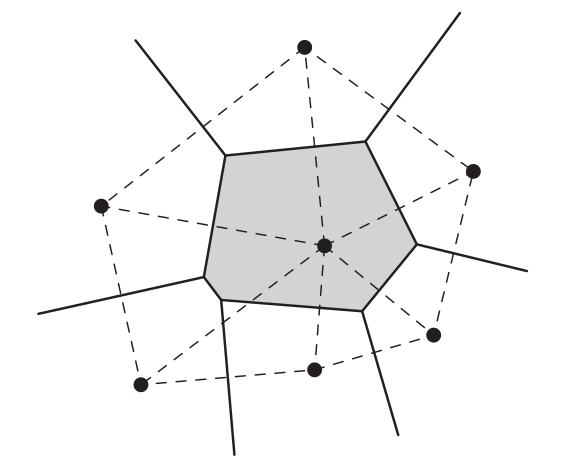
\includegraphics[scale=0.35]{img/voronoi_delone.png}
			\caption{Celda de Voronoi mostrada como línea continua, Celda de Delone como línea punteada. Figura 2.1. de \cite{b1}.}
			\label{voronoi_delone}
		\end{figure}
	\item La Celda de Wigner$-$Seitz es un tipo de celda primitiva (celda con volumen mínimo) trazada por un método llamado igual que la celda (figura \ref{wigner-seitz}).
		\begin{figure}[H]
			\centering
			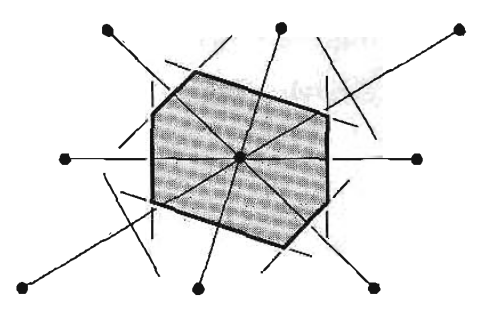
\includegraphics[scale=0.35]{img/wigner_seitz.png}
			\caption{Para trazar la Celda de Wigner$-$Seitz, se trazan líneas desde un punto previamente dado hasta todos los puntos más cercanos. En el punto medio de dichas líneas se trazan unas nuevas (líneas o planos) normales a ellas, el volumen/área más pequeño encerrado por esas líneas/planos, es la celda de Wigner$-$Seitz. Figura 4, capítulo 1, de \cite{b2}.}
			\label{wigner-seitz}
		\end{figure}
	Mientras que la Primera Zona de Brillouin es la Celda de Wigner$-$Seitz en la red recíproca.
	\item 
	\item Para los planos $(111)$, $(110)$ se tiene la siguiente figura (primera y última imagen)
		\begin{figure}[H]
			\centering
			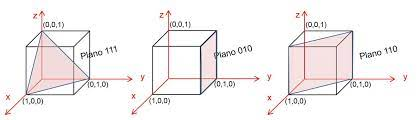
\includegraphics[scale=0.8]{img/planes.jpeg}
			\caption{Planos en una red cúbica simple. Imagen extraída de \cite{b3}.}
			\label{planes}
		\end{figure}
		Con esto podemos encontrar los vectores normales a cada uno de los planos (apuntando al primer octante). Los puntos de interes son
		$$
			\left.\begin{array}{cc}
				P_1 = (1,0,0) & Q_1 = (0,1,0) \\
				P_2 = (0,0,1) & Q_2 = (0,1,1) \\ 
				P_3 = (0,1,0) & Q_3 = (1,0,0) \\
				 & \\
				P_3 P_1 = (-1,1,0) & Q_3 Q_1 = (1,-1,0) \\
				P_2 P_1 = (-1,0,1) & Q_2 Q_1 = (0,0,1) \\
				\downarrow & \downarrow \\
				P_3 P_1 \cp P_2 P_1 & Q_2 Q_1 \cp Q_3 Q_1 \\
				\downarrow & \downarrow \\
				N_P = (1,1,1) & N_Q = (1,1,0),
			\end{array}\right.
		$$
		Con los vectores normales encontrados, utilizando el producto punto para encontrar el ángulo, se tiene
		$$ \theta = \arccos{\frac{\abs{N_P \cdot N_Q}}{\abs{N_P} \abs{N_Q}}} = 35.26^o . $$
	\item Teniendo la forma de empaquetamiendo atómico para una red $FCC$.
		\begin{figure}[H]
			\centering
			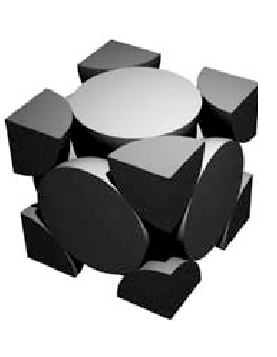
\includegraphics[scale=0.35]{img/fcc.png}
			\caption{$FCC$.}
			\label{fcc}
		\end{figure}
		Como se puede ver en la figura \ref{fcc} el número de átomos por celda es $N_{a} = 6*\frac{1}{2} + 8*\frac{1}{8}$. El radio del átomo en términos del lado de cubo es $4R = \sqrt{2} a$, entonces el volumen del átomo es
			$$ V_a = \frac{\sqrt{2}}{24} \pi a^3; $$
		por lo que, el factor de empaquetamiento atómico para una red $FCC$ es
			$$ APF = N_a \frac{V_a}{V_c} = 4*\frac{\frac{\sqrt{2}}{24} \pi a^3}{a^3} = \frac{1}{6} \sqrt{2} \pi = 0.74. $$
	\item Tomando como idea el cálculo de la red recíproca de un \textit{sc}, cuyos vectores recíprocos son $\vb{b_1} = \qty(\flatfrac{2\pi}{a})\vx$, $\vb{b_2} = \qty(\flatfrac{2\pi}{a})\vy$ y $\vb{b_3} = \qty(\flatfrac{2\pi}{a})\vz$; y, sabiendo que una red unidimencional es equivalente a un lado del cubo, entonces, dicha red existe y es de la forma $\vb{b} = \qty(\flatfrac{2\pi}{a}) \vu{u}$. El hipervolumen de la primera zona de Brillouin es, en el caso de una dimensión, una longitud dada por los dos vectores más pequeños en la red, i.e. $\vb{b}$, $-\vb{b}$, cuyos bisectores son $-\frac{\pi}{a}$ y $\frac{\pi}{a}$; por lo que, el hipervolumen de la primera zona de Brillouin es $\flatfrac{2\pi}{a}$.
	\item El Hierro tiene una red cristalina centrada en el cuerpo (bcc), mientras que el Níquel presenta una red cristalina centrada en las caras (fcc). Entonces, encontrando la red recíproca del Hierro se tienen los vectores primitivos
		$$ a_1 = \frac{1}{2} a\qty(-\vx + \vy + \vz), \qquad a_2 = \frac{1}{2} a\qty(\vx - \vy + \vz), \qquad a_3 = \frac{1}{2} a\qty(\vx + \vy - \vz). $$
	Entonces, construimos los vectores de la red recíproca
		$$ b_1 = 2\pi \frac{a_2 \cp a_3}{a_1 \cdot a_2 \cp a_3}, \qquad b_2 = 2\pi \frac{a_3 \cp a_1}{a_1 \cdot a_2 \cp a_3}, \qquad b_3 = 2\pi \frac{a_1 \cp a_2}{a_1 \cdot a_2 \cp a_3}. $$
	Con ayuda de \textit{Mathematica} (función \texttt{Cross[]}) encontramos cada uno de los productos cruz
		\begin{align*}
			a_2 \cp a_3 &= \frac{1}{2} a(\vy + \vz) \\
			a_3 \cp a_1 &= \frac{1}{2} a(\vx + \vz) \\
			a_1 \cp a_2 &= \frac{1}{2} a(\vy + \vy) \\
			a_1 \cdot a_2 \cp a_3 &= \frac{1}{2} a, 
		\end{align*}
	entonces, sustituyendo en los vectores de la red recíproca se tiene
		\begin{align*}
			b_1 &= \frac{2\pi}{a} (\vy + \vz) \\
			b_2 &= \frac{2\pi}{a} (\vx + \vz) \\
			b_3 &= \frac{2\pi}{a} (\vx + \vy).
		\end{align*}
	Los cuales son equivalentes a los vectores primitivos para una red fcc, por ende a la red cristalina del Níquel.
	\item 
\end{enumerate}

\subsection{Problema 2}
\subsection{Problema 3}
Según el libro \cite{b1}, el factor de forma atómica, lo podemos escribir como	
	$$ f(k) = \frac{4\pi}{e} \int \dd{r} r^2 \rho (r) \frac{\sin{kr}}{kr}, $$
reemplazando $\rho (r) = \frac{1}{\pi a_o ^3} e^{\flatfrac{-2r}{a_o}}$ se tiene
	$$ f(k) = \frac{4}{kea_o ^3} \underbrace{\int _0 ^\infty r\sin{kr} e^{\flatfrac{-2r}{a_o}} \dd{r}}_{\text{Utilizando Mathematica}} = \frac{4}{kea_o ^3} \qty(\frac{4a_o ^3 k}{(4 + k^2 a_o ^2)^2}) = \frac{16}{e\qty(4 + k^2 a_o ^2)^2}. $$



\section{Parcial 2}
\label{sec:parcial2}

\subsection{Problema 1}
Para el oscilador armónico cuántico se tiene el hamiltoniano
\begin{equation}
	H = \frac{p^2}{2m} + \frac{1}{2} m\omega ^2 q^2 , \label{hamilQAO}
\end{equation}
también las relaciones adensionales $Q^2 = \flatfrac{m\omega q^2}{\hbar}$ y $P^2 = \flatfrac{p^2}{m\hbar \omega}$. Los operadores $q$ y $p$ satisfacen $[q,p] = i\hbar$ y se tienen los operadores de creación y aniquilación
	$$ a = \frac{1}{\sqrt{2}} (Q + iP), \qquad a^\dagger = \frac{1}{\sqrt{2}} (Q - iP), $$
con el operador número definido como $N = a^\dagger a$.
\begin{enumerate}[a)]
	\item Dadas las relaciones adimensionales $Q^2$ y $P^2$, se tienen de forma lineal $Q = \sqrt{\flatfrac{m\omega}{\hbar}} q$ y $P = \flatfrac{1}{\sqrt{m\omega \hbar}} p$, entonces, el conmutaror $[Q,P]$ es
		$$ [Q,P] = \sqrt{\frac{m\omega}{\hbar}} \sqrt{\frac{1}{m\omega \hbar}} \underbrace{[q,p]}_{i\hbar} = \boxed{ i\hbar . } $$
	\item Para el conmutador entre los operadores de creación y aniquilación se tiene
		$$ [a,a^\dagger] = \frac{1}{2} \qty([Q,Q] + i[P,Q] - i[Q,P] + [P,P]) = \frac{1}{2} ( 1 + 1 ) = \boxed{1.} $$
	\item El hamiltoniano en terminos de las relaciones adimensionales es
		$$ H = \frac{\hbar \omega}{2} \qty(P^2 + Q^2), $$
	y, utilizando mathematica (para facilitar los cálculos), los operadores $Q$, $P$ en términos de los operadores aniquilación y creación, son
		$$ Q = \frac{1}{\sqrt{2}} \qty(a + a^\dagger), \qquad P = -\frac{i}{\sqrt{2}} \qty(a - a^\dagger). $$
	Entonces
		$$ Q^2 = \frac{1}{2} \qty(a^2 + a^{\dagger ^2} + aa^\dagger + a^\dagger a), \qquad P^2 = -\frac{1}{2} (a^2 + a^{\dagger ^2} - aa^\dagger - a^\dagger a). $$
	Sustituyendo en el hamiltoniano encontrado este inciso
		$$ H = \boxed{ \frac{\hbar \omega}{2} \qty(aa^\dagger + a^\dagger a). } $$
	\item Para este inciso, utilizamos la siguiente propiedad de los conmutadores $[AB,C] = A[B,C] + [A,C]B$, entonces
		$$ [N,a] = a^\dagger [a,a] + \underbrace{[a^\dagger ,a]}_{-1} a = \boxed{ -a. } $$
		$$ [N,a^\dagger] = a^\dagger [a,a^\dagger] + [a^\dagger ,a^\dagger] a = \boxed{ -a^\dagger .} $$
\end{enumerate}



\subsection{Problema 2}


\subsection{Problema 3}
La energía cinética individual está dada como $\frac{1}{2} M \dot{u}_s ^2$, y la fuerza entre los átomos contiguos de la red tiene la forma de la ley de Hooke $-C (u_s - u_{s + 1})$ (solo tomando el estiramiento). Su potencial esta dado por $\frac{1}{2} C (u_s - u_{s + 1})^2$, esto se extiende a toda la red. Con esto, la energía total esta dada por
	$$ E = \frac{1}{2} M \dot{u}_s ^2 + \frac{1}{2} C (u_s - u_{s + 1})^2. $$
Para encontrar la energía potencial y cinética promediada en el tiempo partimos de sustituir en la energía potencial la función $u_s$, entonces se tiene
	\begin{align*}
		u_s - u_{s + 1} &= u\cos{\qty(\omega t - ska)} - u\cos{\qty(\omega t - (s+1)ka)} \\
		&= u\cos{\qty(\omega t - ska)} - \qty[u\cos{\qty(\omega t - ska)} \cos{ka} - u\sin{\qty(\omega t - ska)} \sin{ka}] \\
		(u_s - u_{s + 1})^2 &= u^2 \cos^2 {\qty(\omega t - ska)} (1 - \cos{ka})^2 + u^2 \sin^2 {\qty(\omega t - ska)} \sin^2 {ka} \\ 
		&- 2u^2 \cos{\qty(\omega t - ska)}\sin{\qty(\omega t - ska)} (1 - \cos{ka})\sin{ka},
	\end{align*}
	sabiendo que $\expval{\sin^2 {x}} + \expval{\cos^2 {x}} = \expval{1} = 1 $ y como para el seno y coseno este valor esperado debe ser igual, entonces $\expval{\sin^2 {x}} = \expval{\cos^2 {x}} = \frac{1}{2}$; además, $\expval{\sin{x} \cos{x}} = 0$. Con esto, calculamos el valor esperado de la energía potencial
	\begin{align*}
		\expval{V} &= \frac{1}{2} u^2 \qty(1 - \cos{ka})^2 + \frac{1}{2} u^2 \sin^2 {ka} = u^2 \qty(1 - \cos{ka}).
	\end{align*}
	Integrando la relación de disperción dada en el intervalo de $0\to k$
		$$ \omega ^2 = \int _0 ^k \frac{2Ca}{M} \sin{ka} \dd{k} = \frac{2C}{M} \qty(1 - \cos{ka}), $$
	sustituyendo en el valor esperado de la energía potencial
		$$ \expval{V} = \frac{1}{4} M\omega ^2 u^2. $$
	Para la energía cinética, derivamos $u_s$ respecto al tiempo $\dot{u}_s = -u\omega \sin{\qty(\omega t - ska)}$, entonces
	\begin{align*}
		\expval{\dot{u}_s ^2} &= u^2 \omega ^2 \sin^2 {\qty(\omega t - ska)} = \frac{1}{2} u^2 \omega ^2 \\
		\expval{T} &= \frac{1}{4} M\omega ^2 u^2,
	\end{align*}
entonces
	$$ \expval{E} = \expval{T} + \expval{V} = \frac{1}{2} M\omega ^2 u^2 . $$
\subsection{Problema 4}
Dado que el potencial es continuo con infinitas derivadas, se cumple el teorema de taylor. En concreto, podemos escribir el potencial como una serie de Maclaurin (porque es alrededor del cero)
	$$ V(r) = V(0) + \frac{V'(0)}{1!} r + \frac{V''(0)}{2!} r^2 \cdots , $$
tomando $V(0) = V'(0) = 0$ y $r\ll 0$; de modo que
	$$ V(r) = \frac{V''(0)}{2} r^2 . $$
Donde el error esta dado por
	$$ \text{Error} = \abs{\frac{V^{(n+1)} (\xi)}{(n + 1)!} r^{n + 1}}, $$
con $\xi \in (0,r)$.

%\section{Examen Final}
%\label{sec:final}
%
%\subsection{Problema 1}
%
%
%
%\subsection{Problema 2}
%
%
%
%
%\subsection{Problema 3}





%\section*{Agradecimientos}
%\label{sec:agradecimientos}


% References
\nocite{*}
\bibliographystyle{IEEEannot}%
\bibliography{references}%

\begin{thebibliography}{00}
\bibitem{b1} Baake, M., \& Grimm, U. (2013). \textit{Aperiodic order (Vol. 1)}. Cambridge University Press.
\bibitem{b2} McEuen, P., \& Kittel, C. (2005). \textit{Introduction to solid state physics.}
\bibitem{b3} UNIVERSIDAD DEL PAÍS VASCO / EUSKAL HERRIKO UNIBERTSITATEA ESCUELA DE INGENIERÍA DE BILBAO / BILBOKO INGENIERITZA ESKOLA. (s/f). Ehu.eus. Recuperado el 26 de noviembre de 2022, de \url{https://ocw.ehu.eus/pluginfile.php/51169/mod_resource/content/0/Tema\%203-Estructura\%20cristalina.pdf}


\end{thebibliography}

\end{document}




%%% Local Variables:
%%% mode: latex
%%% TeX-master: t
%%% End:
